\subsection{Nginx+uWsgi+KeyStone的部署模式}

通常的情况下,KeyStone一般使用httpd或者本身的wsgi脚本进行启动。不过,在生产环境中,
为了追求高性能,一般采用httpd的方式,将KeyStone挂载到httpd,复用httpd的高性能,从而
提升keystone的性能,增加抗压的能力。但是,在高并发的情况下,这种模式出现了一些问题。
Httpd的mod\_wsgi插件在实际的使用过程中,会出现KeyStone占用的内存没有释放。为了解决
这个问题,可以在某些情况下,采用Nginx+uWsgi的方式来部署KeyStone,解决内存泄漏的问题。

\subsubsection{安装相关的依赖}
\begin{code-block}{bash}
yum install nginx uwsgi uwsgi-plugin-python
\end{code-block}

\subsubsection{配置uWsgi主进程}
\begin{code-block}{bash}
mv /etc/uwsgi.ini /etc/uwsgi.ini_bak
mkdir -p /var/log/uwsgi
cat >/etc/uwsgi.ini<<EOF
[uwsgi]
uid = root
gid = root
socket = /var/run/uwsgi/uwsgi.socket
pidfile = /var/run/uwsgi/uwsgi.pid
emperor = /etc/uwsgi.d
master = true
autoload = true
log-date = true
logto = /var/log/uwsgi/uwsgi-emperor.log
EOF
\end{code-block}

\subsubsection{设置uWsgi的keystone脚本}
\begin{code-block}{bash}
cat >/etc/uwsgi.d/keystone-admin.ini<<EOF
[uwsgi]
chmod-socket = 666
master = true
plugin = python
socket = /run/uwsgi/keystone-admin.sock
thunder-lock = true
workers = 4
wsgi-file = /usr/bin/keystone-wsgi-admin
EOF

cat >/etc/uwsgi.d/keystone-public.ini<<EOF
[uwsgi]
chmod-socket = 666
master = true
plugin = python
socket = /run/uwsgi/keystone-public.sock
thunder-lock = true
workers = 4
wsgi-file = /usr/bin/keystone-wsgi-public
EOF
\end{code-block}

\subsubsection{校验uWsgi加载KeyStone}
\begin{code-block}{bash}
systemctl start uwsgi
systemctl status uwsgi
\end{code-block}

如果能够看到如图 \nameref{fig:uwsgi}的输出,则说明uWsgi和KeyStone整合完毕.接下来就是整合Nginx了.
\begin{figure}[H]
  \centering
  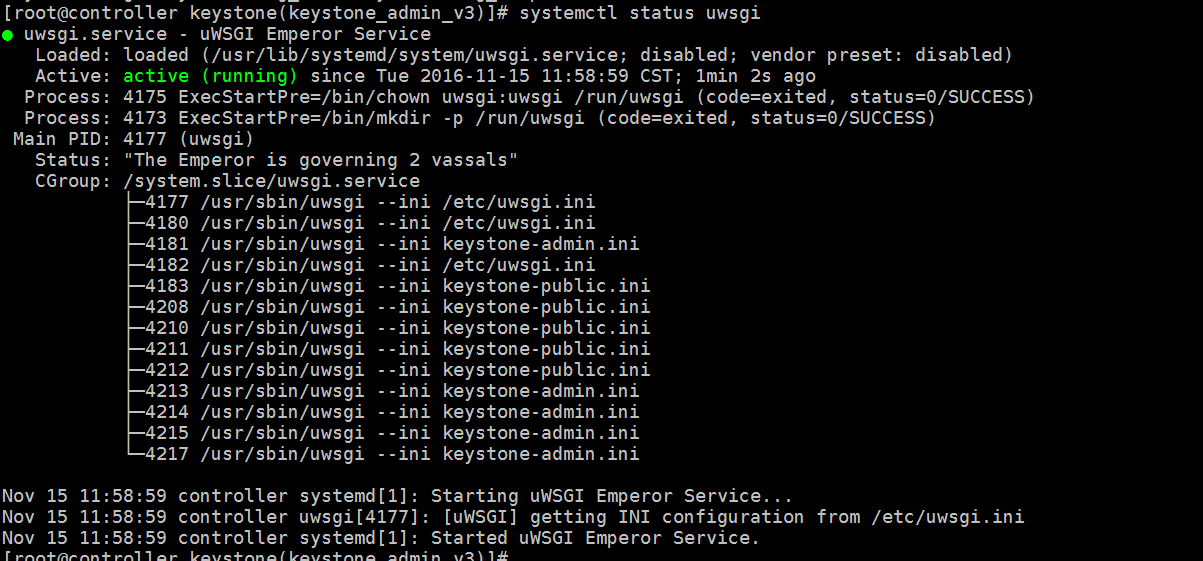
\includegraphics[width=\linewidth]{uwsgi.png}
  \caption{uWsgi加载KeyStone}
  \label{fig:uwsgi}
\end{figure}

\subsubsection{配置Nginx}
添加KeyStone的Nginx支持
\begin{code-block}{bash}
cat >/etc/nginx/conf.d/keystone.conf<<EOF
server {
  listen                *:35357 ;
  server_name           keystone.com;
  access_log            /var/log/nginx/keystone_wsgi_admin.access.log;
  error_log             /var/log/nginx/keystone_wsgi_admin.error.log;
  location / {
    uwsgi_pass       unix:///run/uwsgi/keystone-admin.sock;
    include          uwsgi_params;
    uwsgi_param      SCRIPT_NAME   "";
  }
}
server {
  listen                *:5000 ;
  server_name           keystone.com;
  access_log            /var/log/nginx/keystone_wsgi_public.access.log;
  error_log             /var/log/nginx/keystone_wsgi_public.error.log;
  location / {
    uwsgi_pass       unix:///run/uwsgi/keystone-public.sock;
    include          uwsgi_params;
    uwsgi_param      SCRIPT_NAME   "";
  }
}
EOF

systemctl start nginx
\end{code-block}

\subsubsection{校验KeyStone配置完成}
\begin{code-block}{bash}
openstack token issue
\end{code-block}
